%----------------------------------------------------------------------------------------
%	7./ Opacity derivation
%----------------------------------------------------------------------------------------
%\section{Opacity derivation}
%\label{se:opacity}

Only a fraction of the signal is transmitted by the atmosphere and
reaches NIKA2 detectors. 
The relation between uncorrected observed flux densities
$\tilde{S}_{\nu}$ and top-of-the-atmosphere flux densities $S_{\nu}$
is parametrized by the zenith opacity $\tau_{\nu}$
and the line-of-sight airmass $x = \left(\sin\delta\right)^{-1}$ ($\delta$ is the elevation), such as
\begin{equation}
\tilde{S}_{\nu} = S_{\nu} \, e^{-\tau_{\nu}  x}.
\label{eq:uncorr_flux}
\end{equation}

An accurate derivation of the opacity condition for each scan is
of outmost importance to retrieve the source signal at the top of the
atmosphere and to ensure low calibration uncertainties.
%Opacity correction uncertainties even prevail in the
%final calibration error budget.
We developed three opacity derivation methods, which are described in
Sect.~\ref{se:opacity_methods}, and extensively tested their
robustness against observing conditions, as presented in
Sect.~\ref{opacity_tests}.


\subsection{Opacity derivation}
\label{se:opacity_methods}

To assess the robustness of our opacity measurements, we have devised
three procedures for the opacity derivation: {\tt taumeter} is
described in Sect~\ref{se:taumeter-method} and relies on measurements
provided by the resident IRAM tau-meter operated at $225~\rm{GHz}$ and
a fit of the opacity estimates in NIKA2 frequency bands by imposing
the flux density stability against atmospheric conditions;
{\tt skydip}, described in Sect~\ref{se:skydip-method}, consists in
using NIKA2 as a taumeter (assuming the resonance frequencies are
linearly related to the total power) by resorting to a series of
skydip scans, the selection of which is addressed in
Sect.~\ref{se:skydip-selection}; {\tt corrected skydip}, presented in
Sect.~\ref{se:corrected-skydip}, is a modifed
version of the {\tt skydip} method that minimizes the dependence of the
estimated top-of-the-atmosphere flux density on the opacity.

All these methods i) do not rely on an atmospheric model nor on any
hypothesis on the atmospheric contents for the sake of robustness, and
ii) do not use the laboratory measurements of the bandpass (see 
Sect.~\ref{se:instru_bandpass}) for more accuracy.  

\subsubsection{{\tt taumeter}}
\label{se:taumeter-method}

The IRAM 30-m telescope facility is equipped with a resident taumeter,
which performs elevation scans at a fixed azimuth and is operated at
225~GHz, to monitor the atmospheric opacity. The IRAM science support
team provides us with time-stamped zenith opacities at $225$~GHz
$\tau_{225}$, as derived from the taumeter measures. The
$\tau_{225}$ estimates come in two different flavours: one relying
on a linear model and the other on an exponential fitting model. They
are then filtered by removing outliers and by thresholding on
goodness-of-fit criteria.
%$0< \tau_{225} <1.2$ and $R^2 > 0.99$, where $R^2$ is the coefficient
%of multiple determination of the $\tau_{225}$
%estimates, which quantifies the goodness of fit of each model.
%Redundant samples and outliers are removed.
Based on IRAM experience, we use the linear filtered $\tau_{225}$
data for the NIKA2 analysis. The time-stamped $\tau_{225}$ estimates,
which are sampled about every 4 minutes, are interpolated to the time
of the NIKA2 scans (we consider the time of the middle of the
scan). For cross-check we also produce a smooth version of time-stamped
$\tau_{225}$ data by
filtering with a running median of 7 samples, which is then
interpolated to the NIKA2 scan times.

We fit the relations between the IRAM
$225\,\rm{GHz}$ taumeter opacities and NIKA2 band pass opacities using
observation of calibration sources which spans a large range of air
masses. This method has the advantages of not relying on
any atmosphere model nor on the bandpass measurements in laboratory.
We use a series of 64 scans of MWC349, which consists of the
baseline selected subset of scans from the 68 available scans for
this source during N2R9.
It constitutes an homogeneous data set in flux density but
heterogeneous in atmospheric conditions: zenith opacities at
$225\,\rm{GHz}$ 
range from 0.08 to 0.32 and elevations from $23$ to $73$
degrees, spanning a large range of air mass as required. NIKA2 opacities
$\tau_\nu$, for $\nu$ corresponding
to Array 1, 2, 3 and the combination of Arrays 1 and 3, are estimated
from the $225\,\rm{GHz}$ taumeter median-filtered exponential-based opacity
estimates $\tau_{225}$ as
\begin{equation}  
  \tau_\nu =  a_\nu^{225}\tau_{225} + b_\nu^{225},          
\end{equation}
where the parameters $a_\nu^{225}$ and $b_\nu^{225}$ are fitted to ensure
that the non-corrected flux densities $\tilde{S}_\nu$ are stable against
$\tau_{225}$ after correction of the atmospheric attenuation by
inversion of Eq.~\ref{eq:uncorr_flux} using 
\begin{equation}  
  S_\nu = \tilde{S}_\nu e^{(a_\nu^{225}\tau_{225} + b_\nu^{225}) \cdot x}.
  \label{eq:opacorr_taumeter}
\end{equation}

\begin{table}[!htbp]
  \begin{center}
    \caption[IRAM taumeter to NIKA2 opacity model]{IRAM taumeter to NIKA2 opacity model.}
    \label{tab:tau225-to-taunika}  
    \begin{tabular}{lrrrr}
      \hline
      \hline
      \noalign{\smallskip}
      Parameters & Array 1 & Array 3  & Array 1$\&$3 & Array 2  \\
      \noalign{\smallskip}
      \hline
      \noalign{\smallskip}
      $a_\nu^{225}$         & $1.94$   &  $1.90$ &  $1.92$ & $0.94$ \\
      $b_\nu^{225}$         & $-0.04$  & $-0.07$ & $-0.06$ & $0.00$ \\
      $\Delta a_\nu^{225}$  & $0.15$  & $0.08$  &  $0.09$ & $0.10$ \\
      $\Delta b_\nu^{225}$  & $0.05$  & $0.03$  & $0.04$ & $0.03$ \\
      \noalign{\smallskip}
      \hline
    \end{tabular}
  \end{center}    
\end{table}

We tested two estimators of the flux stability. The first one relies
on minimising the standard deviation of the measured-to-median flux
densities ratio after correction of the opacity using
Eq.~\ref{eq:opacorr_taumeter}. The second one consists in rewriting
the rms minimisation as an unweighted $\chi^2$ minimisation using:
\begin{equation}
\chi^2 = \sum_{i=1}^{N} \frac{1}{\sigma^2} \, \left( \frac{S_\nu}{Med(S_\nu)} -1 \right)^2,  
\end{equation}
where $\sigma$ is the rms error of the flux density estimates. Note
that these estimators do not depend on
the absolute scale of the flux density of the source. Both estimators
yield consistent results that are combined and gathered in
Table.~\ref{tab:tau225-to-taunika}. The quoted errors
$\Delta a_\nu^{225}$ and $\Delta b_\nu^{225}$ are 1-$\sigma$ errors of
the fit.

Because the IRAM tau-meter observes at a fixed azimuth, the
taumeter-based opacities are not exactly the line-of-sight opacities for
the observation scans. As this will be verified in
Sect.~\ref{se:photometry}, this induces larger rms errors of
the top-of-the-atmosphere flux density estimates with respect to
opacity correction methods that relies on skydip-based measurements using
NIKA2 instrument itself. The taumeter-based method will thus be used
as an alternative method in case of i) failure of the NIKA2 skydip-based
methods and ii) to perform consistency checks.



\subsubsection{NIKA2 skydip-based method}
\label{se:skydip-method}

The NIKA2 {\tt skydip} method for the opacity derivation consists in
using the NIKA2 instrument as a tau-meter via a total-power
technique. This technique, which was successfully tested with
NIKA~\citep{Catalano2014}, relies on the assumption that the
resonance frequency of each KID varies linearly with the total
power. First, we have to calibrate the relationship between total
power and opacity. Then we can use this calibration to measure the
opacity during a given scan. Using this procedure we thus directly
derive an opacity integrated in the NIKA2 bandpasses and in the
line-of-sight of the observing scan.

First, we detail the opacity calibration. For each KID $k$, the
absolute value of the resonance frequency $f_{reso}^k$ moves with the
atmospheric transmission according to
%
\begin{equation}
f_{reso}^k  = c_0^k - c_1^k T_{atm}[1-e^{-\tau x}]
\label{eq:skydip}
\end{equation}
%
where $c_0^k$ is a constant equal to the resonance frequency at zero
opacity, $c_1^k$ is the calibration conversion factor in Hz$/$K,
$T_{atm}$ is the temperature of the atmosphere, $\tau$ the zenith
opacity and $\delta$ the elevation of the
telescope.  By assuming a homogeneous plane-parallel atmosphere, the
airmass $x$ is defined from the elevation as $x =
\left(\sin\delta\right)^{-1}$ (we neglect the Earth sphericity).
We take $T_{atm}$ as a constant at 270~K. However, the opacity is
expected to slightly depend on the atmospheric temperature. For
example, in poor weather conditions (6 mm of water vapor contents),
the zenith opacity in the $1~\rm{mm}$ observing bands can vary by
about 10\% for temperature variations of 10~K. The
effect of the temperature variations on the final
calibration of NIKA2 response to the sky load is mitigated by using
several dedicated observation scans regularly distributed all along an
observation campaign.
%
\begin{figure}[!thbp]
\begin{center}
\includegraphics[trim={9cm 0cm 0cm 6.5cm}, clip=true, width=\linewidth]{Figures/test_allskd4_N2R9v5_5-crop.pdf}
\caption[]{Example of the global skydip fit for a KID.
Each square point represents one step in a skydip (made of eleven
elevation steps). 12 skydips are used together spanning zenith
opacities from 0.15 to 0.50. The horizontal axis gives the sky
effective temperature $T_{atm}[1-e^{-\tau x}]$ where $\tau$ is the
skydip zenith opacity found in the fit. The vertical axis shows the
resonance frequency of the KID. The blue line is the expected linear
fit using the found $c_0^k$ and $c_1^k$ coefficients (see
Eq.~\ref{eq:skydip}).}
\label{fig:skydipfitexample}
\end{center}
\end{figure}

The $c_0^k$ and $c_1^k$ are determined using {\tt skydip} scans, which
consist in moving the telescope in elevation step by step, as
defined in Sect.~\ref{se:skydip}. For each KID, the evolution
of $f_{reso}$ is monitored as a function of the airmass in each
elevation step to perform a joint fit of the zenith opacity $\tau$ and
the $c_0^k$ and $c_1^k$ coefficients.
%The acquisition time spent on each elevation step, which is of about
%twenty seconds, is chosen to reduce the error in the determination of
%$f_{reso}$.
All skydips, obtained under various opacity conditions, are analysed
together to break the degeneracy between the opacity and the
responsivity ($c_1^k$). The degeneracy occurs mostly for low opacity
conditions for which we can only determine the combination
$c_1^k \tau x$. The procedure has two steps. First, all the skydips
are analysed individually to extract $f_{reso}^k$ for each
stable elevation and each KID. Secondly, a simultaneous fit is done
for all parameters (one $\tau$ per skydip, and a set of $c_0^k$ and
$c_1^k$ for all KIDs). Fig~\ref{fig:skydipfitexample} illustrates the
fitting procedure.  Error bars on $\tau$ are estimated by doing this
procedure
on blocks of 40 KIDs only and getting a dispersion on the resulting
$\tau$ from the different blocks. Usually the dispersion comes out as
$4\times 10^{-3}$ at 1~mm and $1\times 10^{-3}$ at 2~mm. Once the
$\tau$ values are estimated for each skydip (as the average over the
blocks), we compute, while fixing the $\tau$, the $c_0$ and $c_1$
final values for each KID with a simple linear fit. We thus retrieve
the coefficients of all the KIDs even though some of them could not
contribute to the $\tau$ determination. We find that the skydip-fitted
$\tau$ values are, as expected, equal between different detectors of
the same array.

By comparing the results of different skydips, we have verified that the
coefficients $c_0$, $c_1$ are stable, within the fit errors, on very
long time scales within a cooldown cycle. The coefficients can thus be
applied to the whole observing campaign in order to recover the
opacity of each scan. Namely, he opacity for each array
$A_i$, $i=\{1, 2, 3\}$ are retrieved for each observation scan by
inverting Eq.~\ref{eq:skydip} as:
\begin{equation}
\tau_{A_i} =   Med\left( -\frac{1}{x} \log\left[ \frac{f_{reso}^k - c_0^k}{c_1^kT_{atm}} +1 \right]\right), 
\end{equation}
where the median is evaluated using all the valid KIDs of Array
$i$. Hence we derive an opacity integrated in the NIKA2 bandpasses and
in the line-of-sight of the source in the considered observation scan.


\subsubsection{Skydip selection}
\label{se:skydip-selection}

The {\tt skydip} opacity derivation requires to have on hands a
sizable amount of {\tt skydip} scans --
typically ten to twenty -- that i) span the whole opacity range and
ii) avoid highly perturbated atmosphere to meet the plane-parallel
atmosphere assumption. To that aim, we perform a skydip
scan twice a day during a scientific campaign. Then the ($c_0$, $c_1$)
determination process relies on a selection of the skydip scans.
%
\begin{figure}[!thbp]
\begin{center}
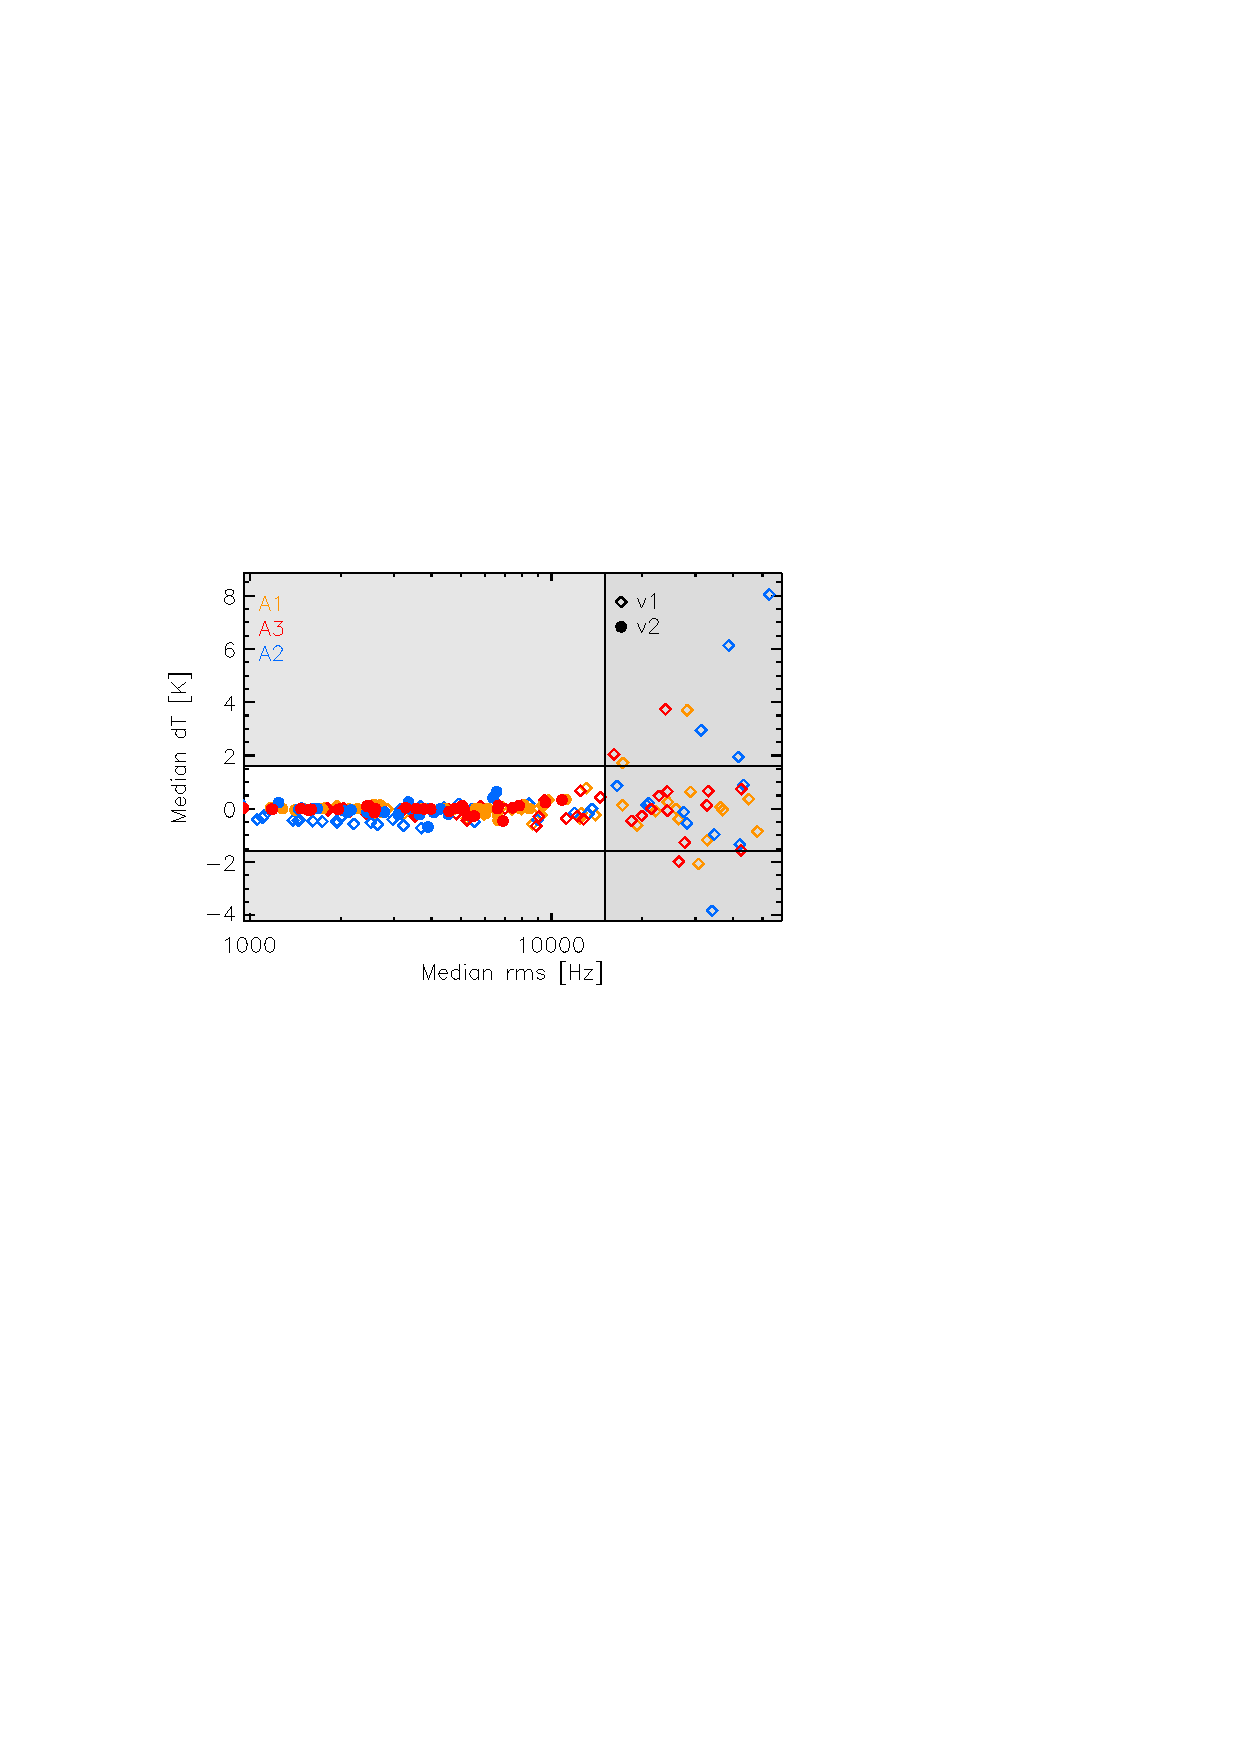
\includegraphics[clip=true,width=\linewidth]{Figures/plot_skydip_selection_two_crit.pdf}
\caption[N2R9 skydip scan selection.]{ Median dT quality-fit criterion
is plotted as a function of the median rms criterion for each skydip
scan of the N2R9 campaign and for the three arrays. Both criteria are
nicely correlated. Empty diamonds show the results of the first
iteration of the skydip coefficient estimation, labeled 'v1', whereas
filled circled show the second iteration, labeled 'v2', for which only the skydips
that met both fit-quality criteria are included.
After the second iteration, all the remaining skydips met the criteria.}
\label{fig:skydipselection}
\end{center}
\end{figure}

For each skydip scan and for each bunch of 40 KIDs, we compute the
difference between the measured KID resonance frequency and the model
given in Eq.~\ref{eq:skydip} taken at the best-fit values of the
($c_0$, $c_1$) parameters. Then we determine two indicators of the fit
quality per skydip. First, the standard deviation of the
measure-to-model difference is calculated over all the KIDs in a
bunch. For each skydip, we evaluate the median rms, which is the
median over the KID bunches of the standard deviation per bunch, given
in Hz. This fit quality indicator is thus also sensitive to the noise
level during the skydip. We therefore devise an additional fit quality
indicator to further measure the bias between measures and model fits.
Namely, for each scan, we compute the average
measure-to-model difference of each KID $k$, labelled $dT_k$, which is
then converted from Hertz to Kelvin using the $c_1$ parameter of the
KID $k$. This cross-calibration allows for assembling the
measure-to-model difference estimates of all the KIDs.
Median $dT$ is the median of $dT_k$ over all the KIDs of an
array. With these two indicators in hands, we discard the skydip scans
that are noisy or that yield a poor fit by applying the selection
criteria that have to be satisfied:

\begin{itemize}
\item Median $\rm{rms} < 1.5 \times 10^{4}~\rm{Hz}$
\item Median $dT < 1.6~\rm{K}$
\end{itemize}

The threshold values have been determined using the set of 44 skydip
scans of N2R9. The Median rms cut corresponds to twice the median of
this quantity per skydip scan, whereas the Median $dT$ cut is twice
the standard deviation of Median $dT$ over the skydips.
N2R9 skydip scan selection is illustrated in
Fig.~\ref{fig:skydipselection}, in
which the agreement between the two fit-quality criteria is clearly
seen.

The ($c_0$, $c_1$) estimation proceeds in two steps: first the
parameters are estimated using all the available skydip scans for a
given campaign, then the estimation is re-iterated using the only
skydip scans that met the fit-quality criteria. After the second
iteration, we check that no extra skydip outlier are left, as shown by
the 'v2' label data points in Fig.~\ref{fig:skydipselection}.
%After
%selection of the skydip scans acquired during the N2R9 campaign, 15
%skydips are kept for the final step of the ($c_0$, $c_1$) fit. 





\subsubsection{{\tt corrected skydip}}
\label{se:corrected-skydip}
